\documentclass[10pt, sans, compress, usenames, dvipsnames, aspectratio=169]{beamer}

%% Import the template configuration
\usepackage[T1]{fontenc}
\usepackage{lmodern}
\usepackage{graphicx}
\usepackage[french]{babel}
\usepackage[utf8]{inputenc}
\usetheme{Warsaw}
\usepackage{wasysym}
\usepackage{tabularx}
\usepackage{hyperref}
\usepackage[absolute,overlay]{textpos}
\setbeamertemplate{navigation symbols}{}
\useoutertheme{infolines}
\useinnertheme{rectangles}
\setbeamertemplate{background canvas}{
\includegraphics[width=\paperwidth,height=\paperheight]{images/ucabackground-16_9.png}}
\usepackage{caption}
\captionsetup{figurename=}
\definecolor{uca01}{HTML}{006E83}
\definecolor{uca02}{HTML}{0096A0}
\definecolor{uca03}{HTML}{006C82}
\definecolor{uca04}{HTML}{0398A1}
\definecolor{uca05}{HTML}{585656}
\definecolor{uca06}{HTML}{438D97}
\definecolor{grisuca}{HTML}{5E5C5C}


\setbeamercolor{palette primary}{bg=uca06}
\setbeamercolor{palette secondary}{bg=uca03}
\setbeamercolor{palette tertiary}{bg=uca04}
\setbeamercolor{palette quaternary}{bg=uca05}
\setbeamercolor{block title}{bg=uca06}
\setbeamercolor{itemize item}{fg=uca03}
\setbeamercolor{itemize subitem}{fg=uca03}
\setbeamercolor{itemize subsubitem}{fg=uca03}


\setbeamercolor{enumerate item}{bg=uca03,fg=uca03}
\setbeamercolor{enumerate subitem}{bg=uca03,fg=uca03}
\setbeamercolor{enumerate subsubitem}{bg=uca03,fg=uca03}
\setbeamercolor{enumerate mini template}{bg=uca03,fg=uca03}
\setbeamercolor{itemize body}{fg=uca03}
\setbeamercolor{itemize subbody}{fg=uca03}
\setbeamercolor{itemize subsubbody}{fg=uca03}
\setbeamercolor{enumerate body}{fg=uca03}
\setbeamercolor{enumerate subbody}{fg=uca03}
\setbeamercolor{enumerate subsubbody}{fg=uca03}

\setbeamercolor{item projected}{bg=uca03}
\setbeamercolor{section in toc}{fg=grisuca}
\setbeamercolor{normal text}{fg=grisuca}



\title{Reproducibility: an old friend, the laboratory notebook }
\subtitle{Better reproducibility with documented code}
\author[Pierre MARIN]{Pierre Marin\\\texttt{pierre.marin@uca.fr}}
\institute{Université Clermont Auvergne, AuBi, Mésocentre}
\date{\today}

\newif\iflattersubsect

% \AtBeginSubsection[] {
%     \iflattersubsect
%     \begin{frame}<beamer>
%     \frametitle{Sommaire} %
%     \tableofcontents[currentsubsection]
%     \end{frame}
%     \fi
%     \lattersubsecttrue
% }


\begin{document}
% titre et sommaire

\begin{frame}
  \titlepage
  \begin{textblock*}{5cm}(2cm,0.5cm) % {block width} (coords)
  
\includegraphics[width=2.3cm,height=1.3cm]{images/logo_ifb.pdf}
  \end{textblock*}
  \begin{textblock*}{5cm}(13cm,0.3cm) % {block width} (coords)
  
\includegraphics[width=1.5cm,height=1.5cm]{images/i2bc.png}
  \end{textblock*}
  \begin{textblock*}{5cm}(2cm,4cm) % {block width} (coords)
  
\includegraphics[width=3.5cm,height=3cm]{images/logoAuBi-2019.pdf}
  \end{textblock*}
  \begin{textblock*}{5cm}(11cm,4.3cm) % {block width} (coords)
  
\includegraphics[width=3cm,height=3cm]{images/mesocentre.png}
  \end{textblock*}
  
\end{frame}
\begin{frame}
  \frametitle{Sommaire}
   \tableofcontents
\end{frame}

% cahier de manip
\section{The laboratory notebook}
\subsection{The aim}
\begin{frame}[<+->]{Paper version}
\begin{textblock*}{10cm}(1cm,2cm) % {block width} (coords)
Laboratory notebook allow to:
\begin{itemize}
	\item Day-to-day recording each step in a process, experiments...
	\item Report on the progress, and scientific experimentations \newline
	from the idea to final conclusions
	\item Keep track of knowledge in a lab
	\item Useful drafting a patent
	\item Proof of anteriority
\end{itemize}
\end{textblock*}
\only<1>{
\begin{textblock*}{10cm}(1cm,3cm) % {block width} (coords)
  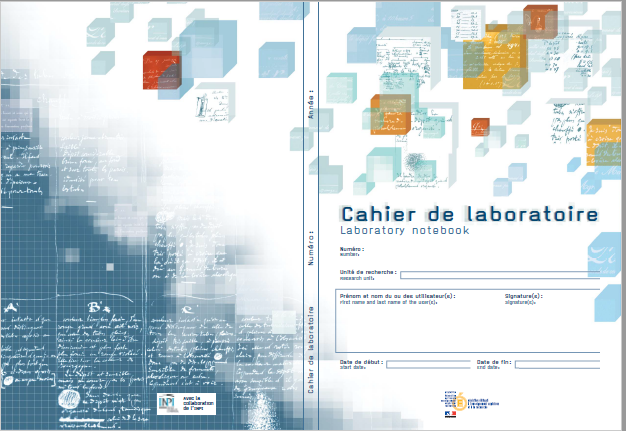
\includegraphics[width=7cm,height=5cm]{images/cahierlabo.png}
 \end{textblock*}
 \begin{textblock*}{10cm}(8cm,3cm) % {block width} (coords)
  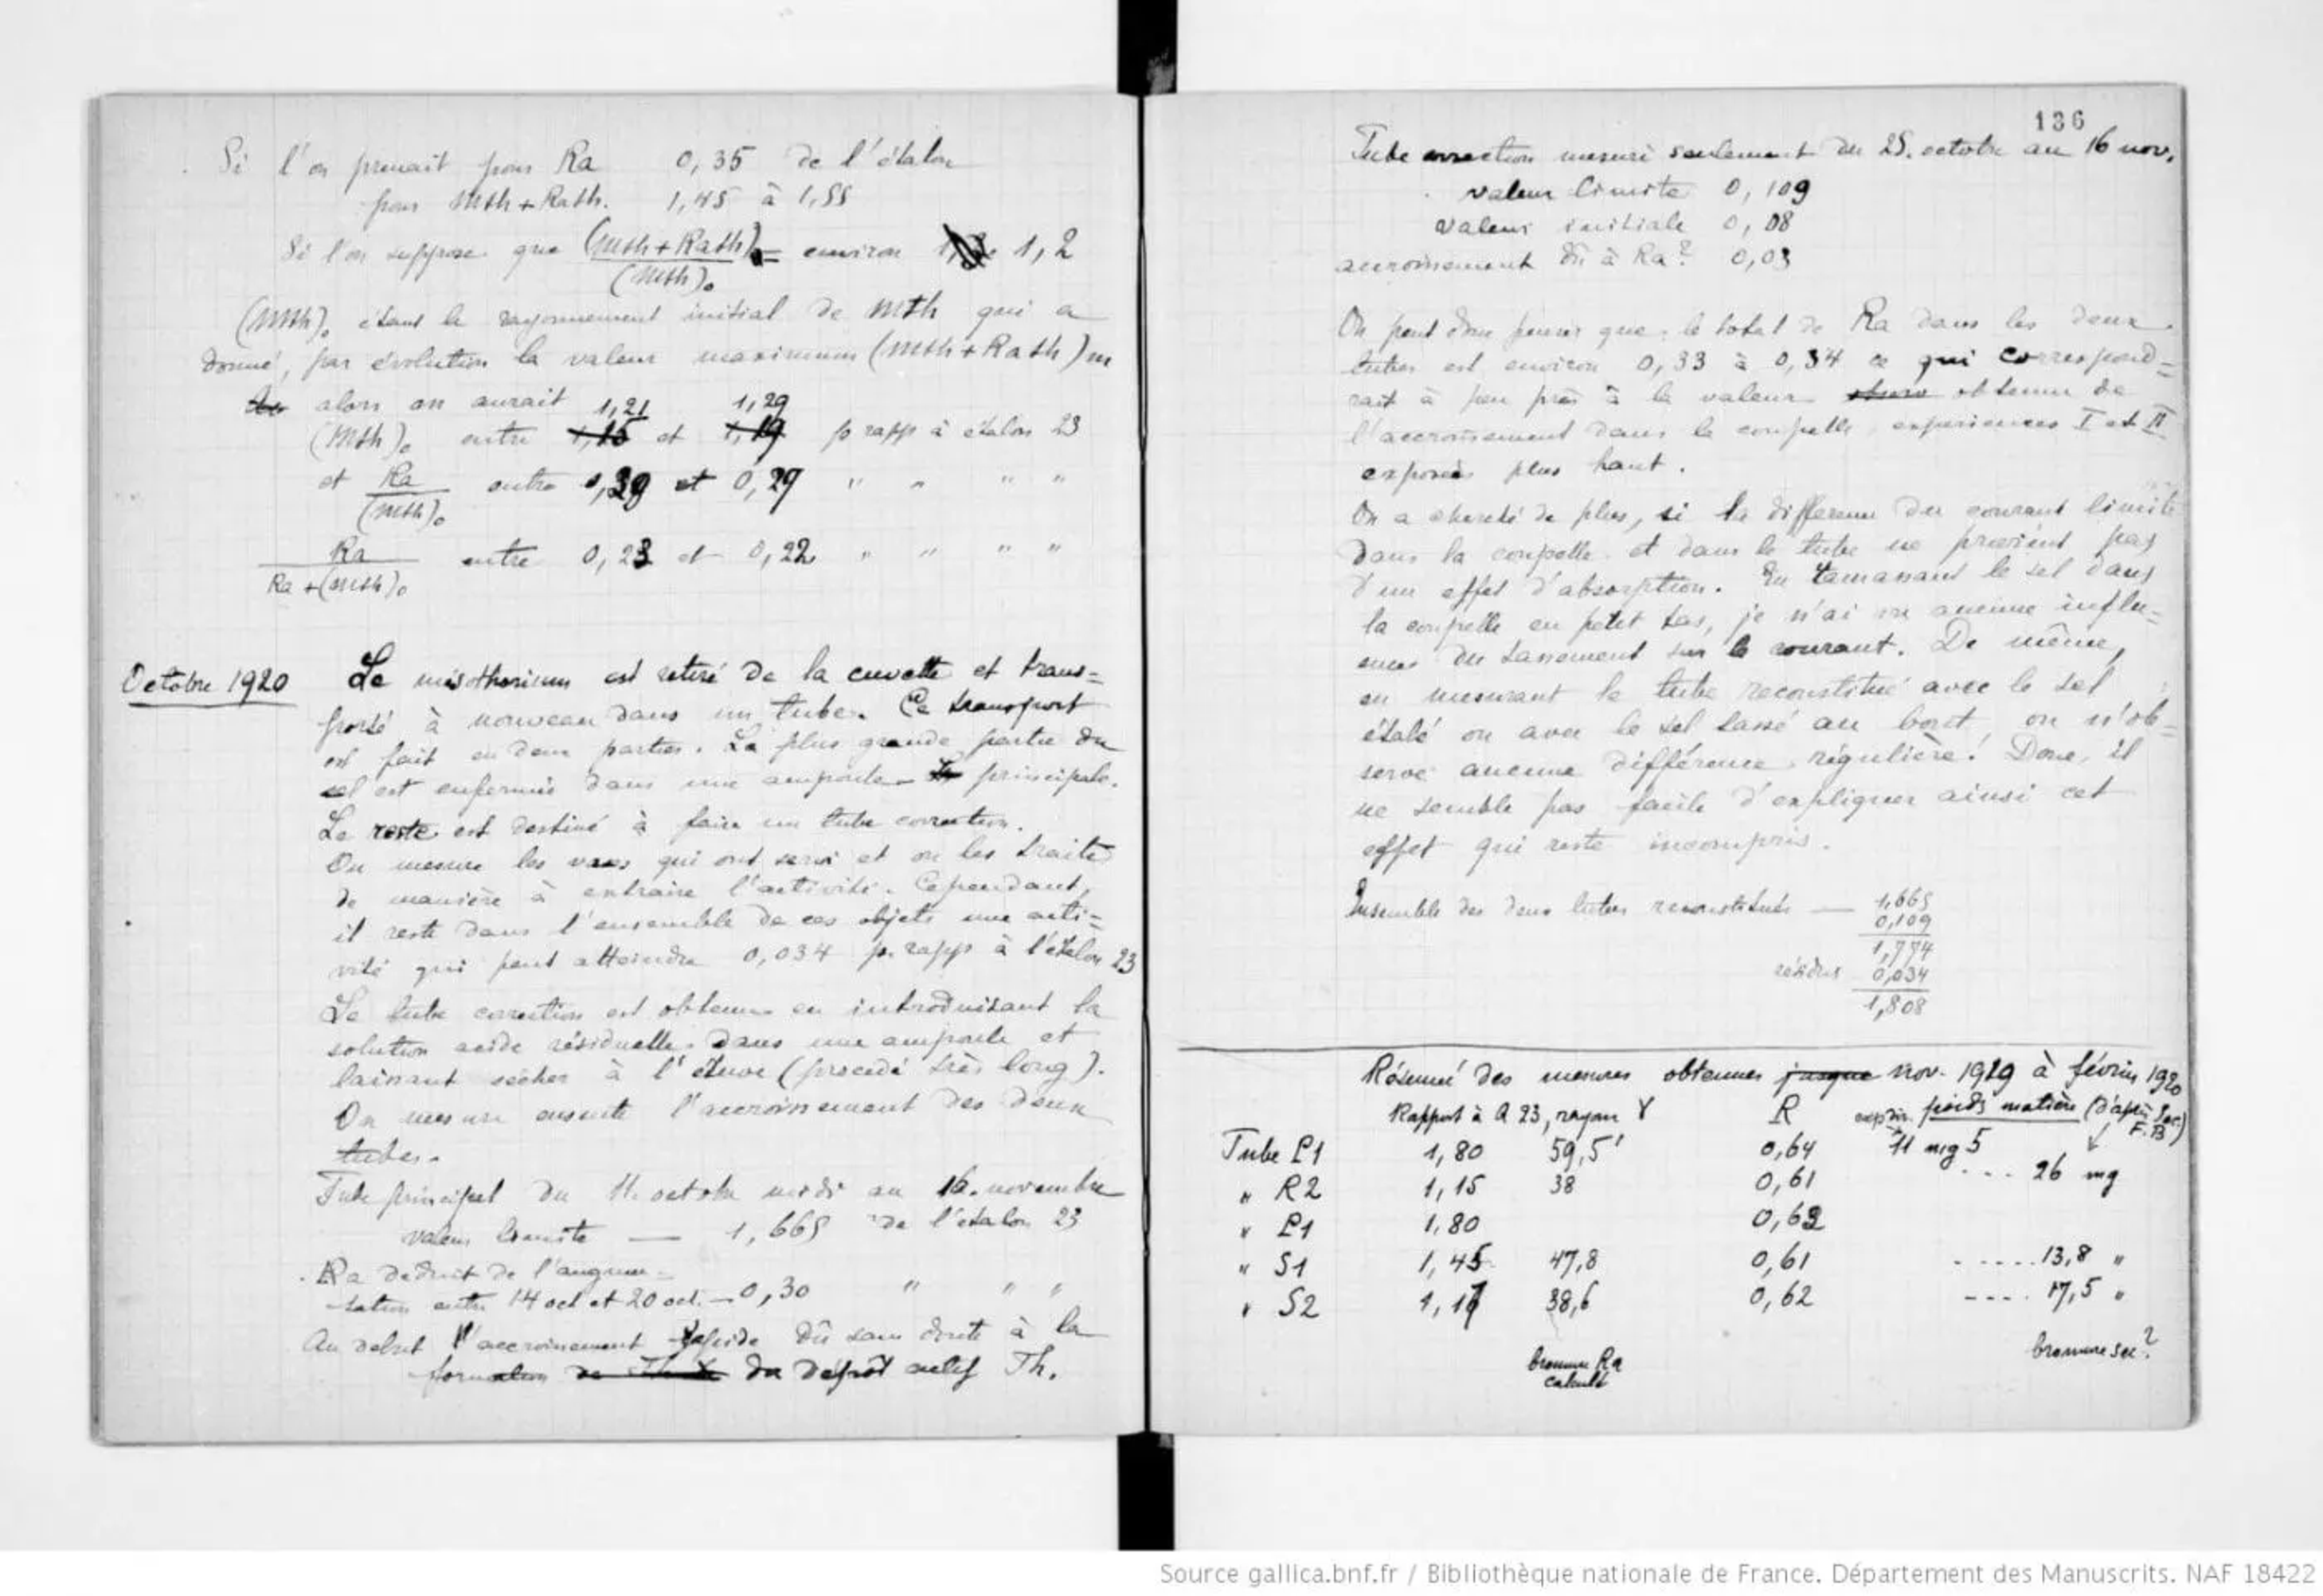
\includegraphics[width=7cm,height=5cm]{images/cahier2.pdf}
 \end{textblock*}}
\end{frame}

\begin{frame}[<+->]{Paper version}
\begin{columns}
\column{.5\textwidth}
This is a legal tool:
 \begin{itemize}
 \item Page numbered in each notebook
 \item Cover page with the owner of the results
 \item Each page contain a part to date, to sign for at least to people
 \end{itemize}
\column{.5\textwidth}
At each research level:
  \begin{itemize}
 \item Researchers
 \item Engineers
 \item Technicians
 \item Students...
 \end{itemize}
\end{columns}
\vspace{1cm}
\onslide<10>{\centering End what's happen for bioinformatic ?}
\end{frame}

\begin{frame}[<+->]{Electronic version}
\onslide<1->{Electronic Laboratory Notebooks (ELN)} \newline
\onslide<1->{Modern LN since 2009 (C.U.R.I.E. Network)}
\only<2>{
\begin{textblock*}{10cm}(9cm,2cm) % {block width} (coords)

\includegraphics[width=3cm,height=1cm]{images/elabftw-logo.png}
\end{textblock*}
\begin{textblock*}{10cm}(0.5cm,4cm) % {block width} (coords)
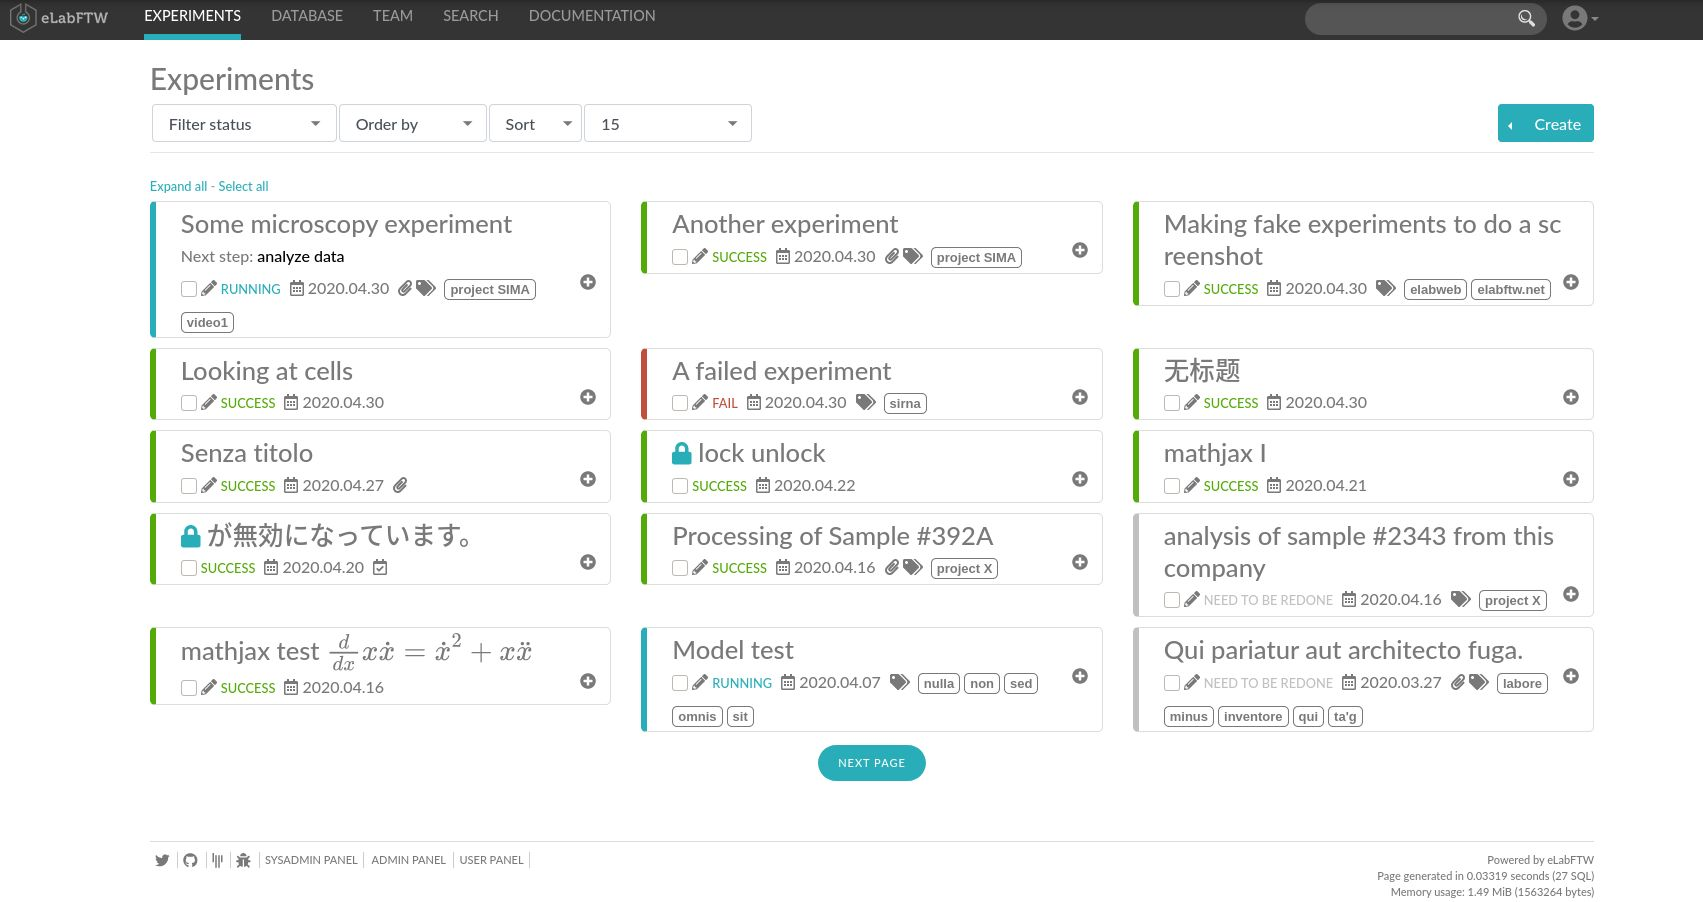
\includegraphics[width=7cm,height=4cm]{images/elabftw1.jpg}
\end{textblock*}
\begin{textblock*}{10cm}(8cm,4cm) % {block width} (coords)
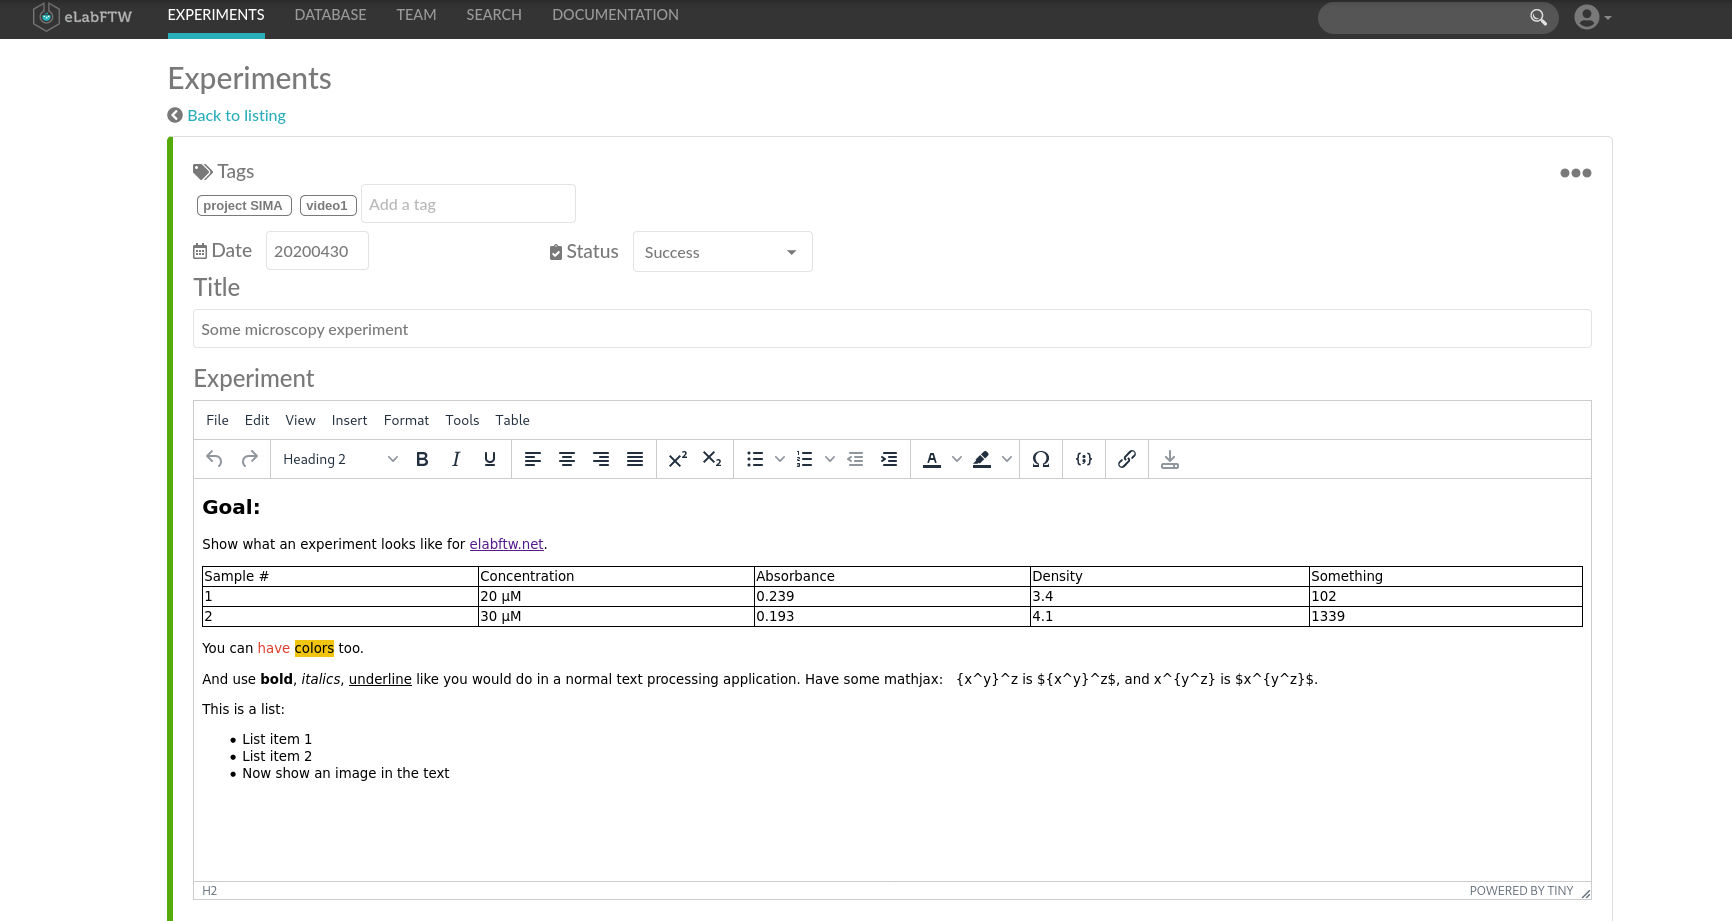
\includegraphics[width=7cm,height=4cm]{images/elabftw2.jpg}
\end{textblock*}}
\onslide<3->{
 \begin{itemize}
 	\item dematerialised
 	\item archivable
 	\item sharable
 	\item secure
 \end{itemize}}
\onslide<4->{
\centering But less and less adapted to recent evolutions of our work \\
\centering We need an electronic tool for individual traceability}
\end{frame}

\begin{frame}{Electronic version}
\only<1>{\centering
\includegraphics[width=10cm,height=7cm]{images/gt_eln.png}}
\only<2>{\centering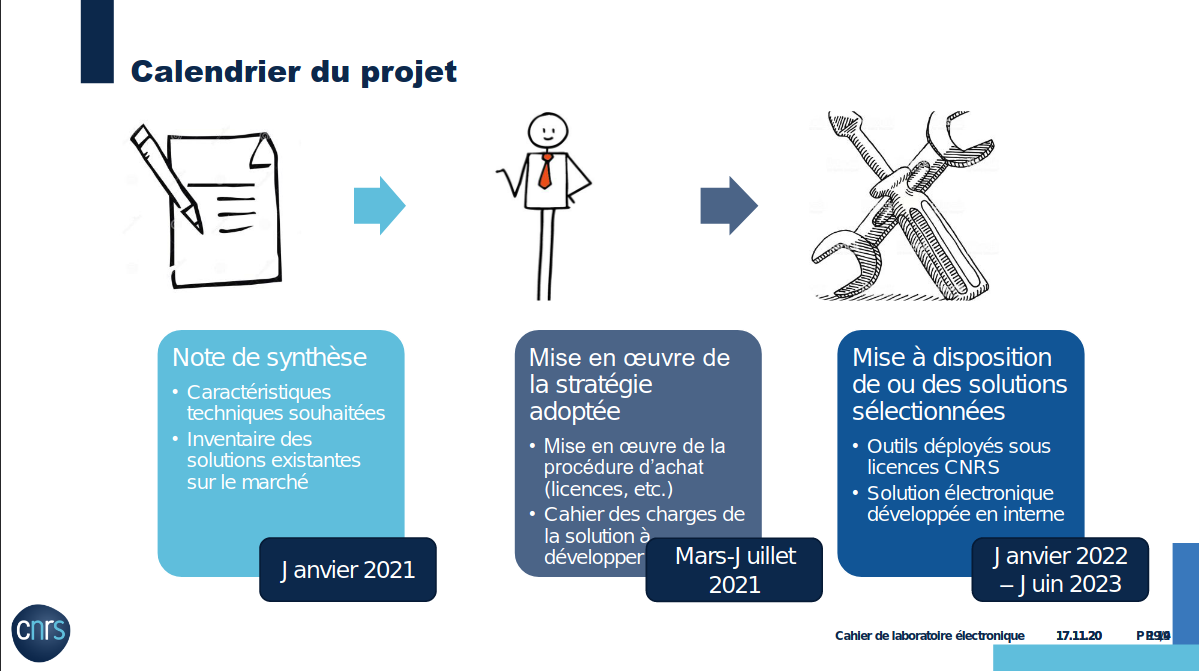
\includegraphics[width=10cm,height=7cm]{images/gt_eln_temp.png}}
\end{frame}


% les notebook
\section{Notebook in bioinformatic}
\subsection*{Literate programming}

\begin{frame}
What is literate programming ?

\emph{
"Let us change our traditional attitude to the construction of programs: \\
Instead of imagining that our main task is to instruct a computer what to do, let us concentrate rather on explaining to humans what we want the computer to do."}
\footnote{Donald E. Knuth, Literate Programming, 1984} 
\newline
\emph{
”Literate programming is a programming paradigm introduced by Donald Knuth in
which a computer program is given an explanation of its logic in a natural language,
such as English, interspersed with snippets of macros and traditional source code,
from which compilable source code can be generated.”}
\footnote{\url{https://en.wikipedia.org/wiki/Literate_programming\# Workflow}}
\end{frame}

\begin{frame}{Literate programming}
Why using literate programming frameworks ?
\begin{itemize}
	\item Labbook
	\item Day-to-day analysis
	\item Make automatic reports
	\item Write scientific article
\end{itemize}
\end{frame}

\begin{frame}{Literate programming}{example}
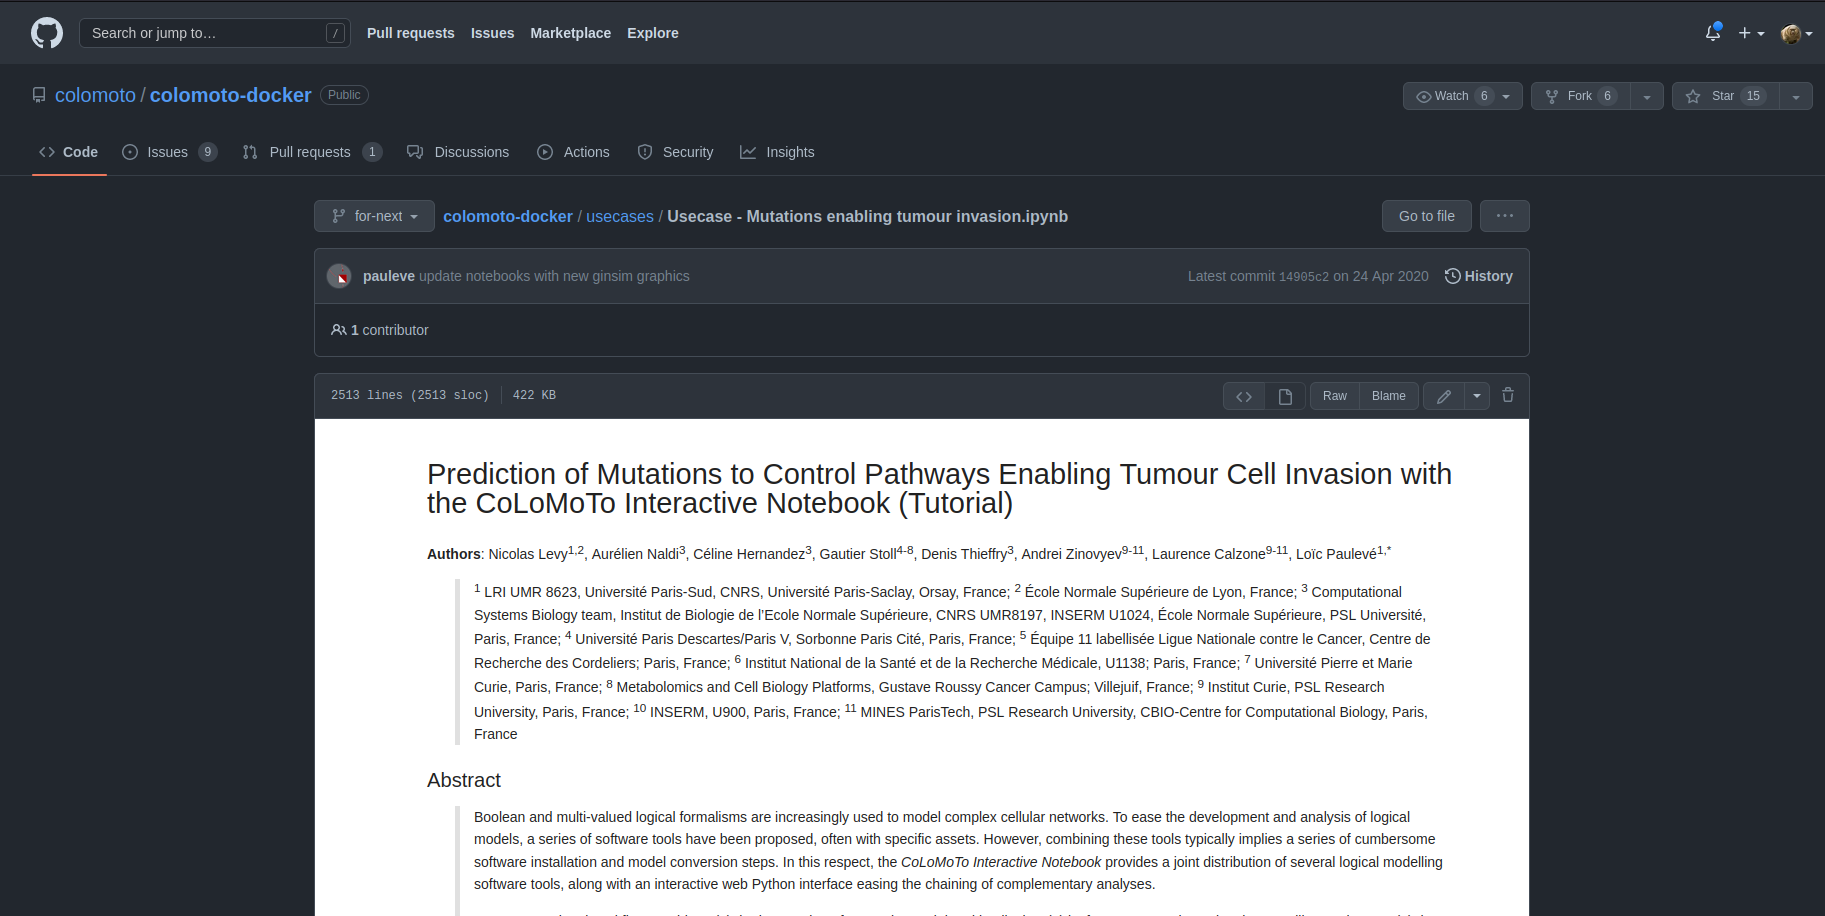
\includegraphics[width=2.3cm,height=1.3cm]{images/colomoto_github.png}
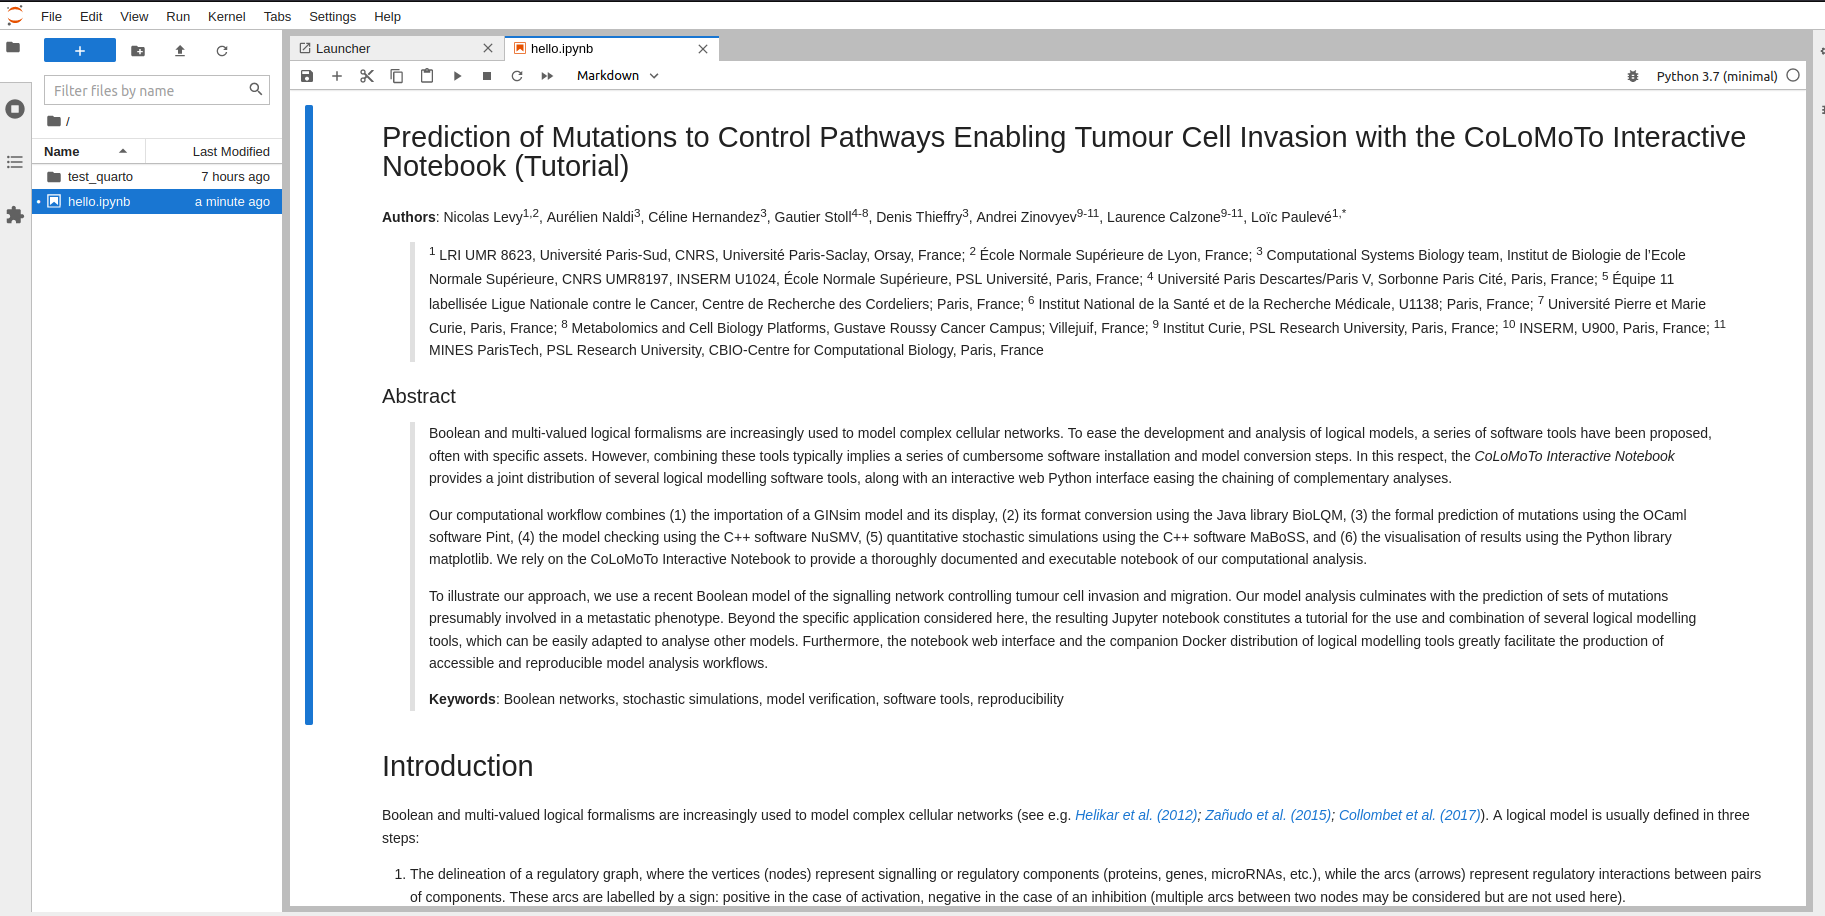
\includegraphics[width=2.3cm,height=1.3cm]{images/colomoto_jupyter.png}

\includegraphics[width=2.3cm,height=1.3cm]{images/colomoto_paper.png}
\href{https://www.frontiersin.org/articles/10.3389/fphys.2018.00787/full}{doi:10.3389/fphys.2018.00787}
\end{frame}

\section{Notebook in bioinformatic}
\subsection*{Literate programming}
\end{document}